In the thesis, all images were artificially generated in a separate component of the described system. Colouring of images was adjusted to the tasks of each experiment, however, the basics of the generation process stayed the same. for this part of the system, a single generated image can be divided into maximally four differently coloured sections, which have the role of a background. Then, in each section, there might be one foreground object placed and it can be a circle, a square, a pentagon or a hexagon. There are also situations in which a foreground object is placed on the area of two sections. In such a way two sets of images were generated, namely a training set containing 200 images and a testing set containing 10 images. When it comes to the size of images, both width, and height was equal to 400px. This means, that during the training process, in which gradient should be computed based on data from every pixel in all images in a training set, it would be required to perform computations for 32 million cases in every single epoch. That is why all the images were subject to the process of superpixel segmentation into roughly 500 superpixels, which limited the number of required computations 320 times. 

For the first experiment that was conducted, the generated images were composed of only three colours: red, green and blue. Figure \ref{fig:test_set_basic} presents six sample images from a testing set that were used to evaluate whether semantic segmentation was successful. A black border around the images is not a part of the given image, it was added for the sake of better visibility. 
\begin{figure}[ht]
    \centering
    \begin{tabular}{ccc}
        \fcolorbox{black}{white}{\includegraphics[width =     0.28\textwidth]{linear_no_noise/test/2.png}} &
        \fcolorbox{black}{white}{\includegraphics[width = 0.28\textwidth]{linear_no_noise/test/3.png}} &
        \fcolorbox{black}{white}{
\includegraphics[width =    0.28\textwidth]{linear_no_noise/test/6.png}} \\ 
        
        \fcolorbox{black}{white}{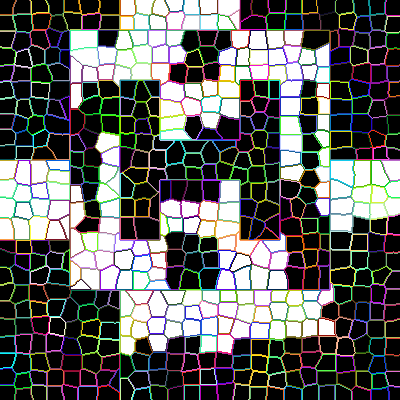
\includegraphics[width = 0.28\textwidth]{linear_no_noise/test/7.png}} &
        \fcolorbox{black}{white}{\includegraphics[width = 0.28\textwidth]{linear_no_noise/test/8.png}} &
        \fcolorbox{black}{white}{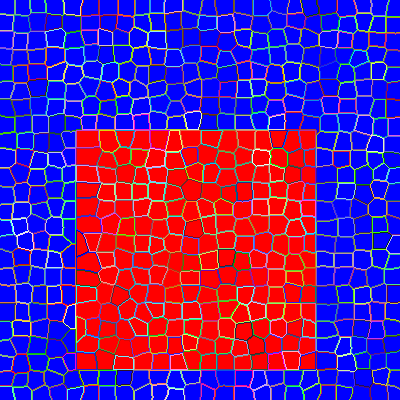
\includegraphics[width = 0.28\textwidth]{linear_no_noise/test/9.png}} 
    \end{tabular}
\caption{Sample test images generated for the first experiment.}
\label{fig:test_set_basic}
\end{figure}

In order to perform the semantic segmentation also a training set is needed, which is composed of images generated in the same way as testing images. However, in order to perform supervised learning not only training images are needed, but also the expected labellings for each of those images. The part of the system described in this chapter performs segmentation of objects into three classes, each specified by one label. All red objects should be assigned to label 0, all green to class 1 and all blue objects should have label 2. For each image from the training set, another image was generated that represents correct labelling of a given image. Pixels with label 0 assigned are painted in black, those with label 1 are white, and pixels with label 2 are grey. Figure \ref{fig:training_set_basic} depicts six pairs of images representing sample training data and their expected labellings.  
\begin{figure}[ht]
    \begin{minipage}{.5\linewidth}
        \begin{tabular}{cc}
            \fcolorbox{black}{white}{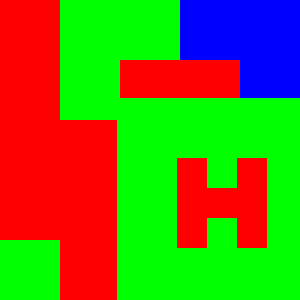
\includegraphics[width = 0.41\textwidth]{linear_no_noise/train/0.png}} &
            \fcolorbox{black}{white}{
\includegraphics[width = 0.41\textwidth]{linear_no_noise/result/0_N.png}} \\ 
            \fcolorbox{black}{white}{\includegraphics[width = 0.41\textwidth]{linear_no_noise/train/2.png}} &
            \fcolorbox{black}{white}{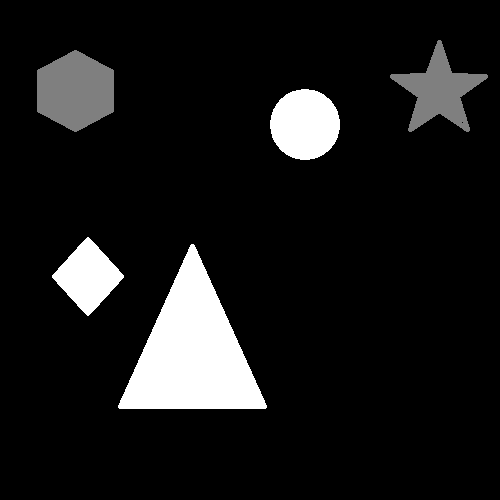
\includegraphics[width = 0.41\textwidth]{linear_no_noise/result/2_N.png}} \\
            \fcolorbox{black}{white}{\includegraphics[width = 0.41\textwidth]{linear_no_noise/train/3.png}} &
            \fcolorbox{black}{white}{
\includegraphics[width = 0.41\textwidth]{linear_no_noise/result/3_N.png}}
        \end{tabular}
    \end{minipage}%
    \begin{minipage}{.5\linewidth}
        \begin{tabular}{cc}
            \fcolorbox{black}{white}{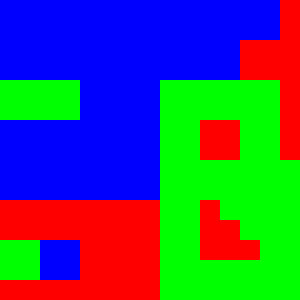
\includegraphics[width = 0.41\textwidth]{linear_no_noise/train/5.png}} &
            \fcolorbox{black}{white}{
\includegraphics[width = 0.41\textwidth]{linear_no_noise/result/5_N.png}} \\ 
            \fcolorbox{black}{white}{\includegraphics[width = 0.41\textwidth]{linear_no_noise/train/8.png}} &
            \fcolorbox{black}{white}{
\includegraphics[width = 0.41\textwidth]{linear_no_noise/result/8_N.png}} \\
            \fcolorbox{black}{white}{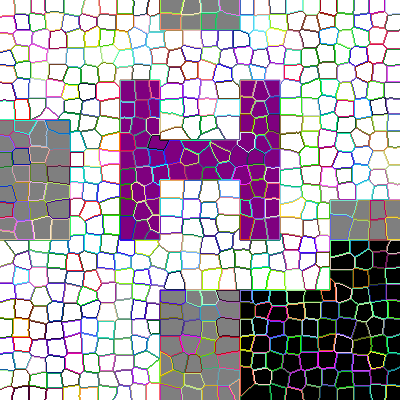
\includegraphics[width = 0.41\textwidth]{linear_no_noise/train/28.png}} &
            \fcolorbox{black}{white}{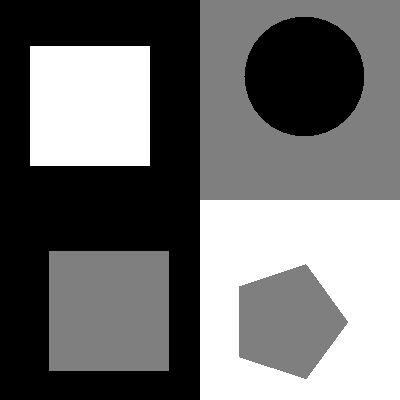
\includegraphics[width = 0.41\textwidth]{linear_no_noise/result/28_N.png}}
        \end{tabular}
    \end{minipage} 
    \caption{Sample train images and their correct labellings generated for the first experiment.}
    \label{fig:training_set_basic}
\end{figure}

For the next experiment, different training and tests sets were required, which were to be composed of images containing not only primary colours but also different shades of them. Those sets were obtained by modifying the already generated images from the first experiment. Firstly, those images were divided into superpixels and then the colour of each superpixel was slightly changed in a random way. Figure \ref{fig:training_set_coloured} presents six pairs of training images with their expected labellings that were generated for the second experiment.
\begin{figure}[ht]
    \begin{minipage}{.5\linewidth}
        \begin{tabular}{cc}
            \fcolorbox{black}{white}{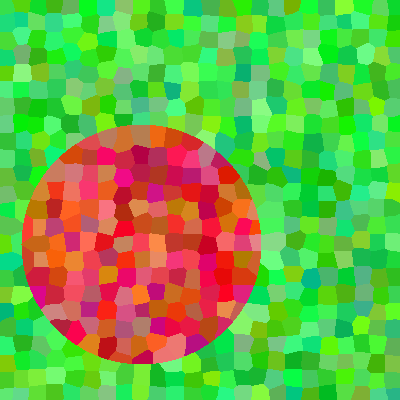
\includegraphics[width = 0.41\textwidth]{linear_coloured/train/115.png}} &
            \fcolorbox{black}{white}{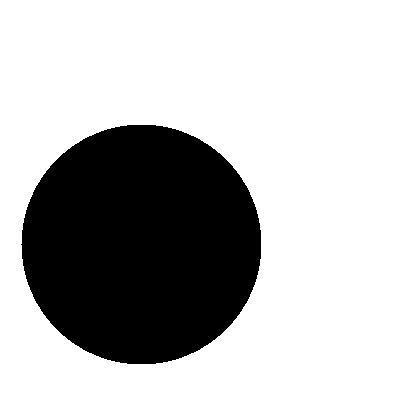
\includegraphics[width = 0.41\textwidth]{linear_coloured/result/115_N.png}} \\
            \fcolorbox{black}{white}{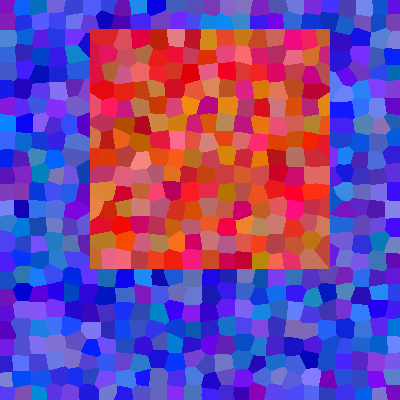
\includegraphics[width = 0.41\textwidth]{linear_coloured/train/116.png}} &
            \fcolorbox{black}{white}{
\includegraphics[width = 0.41\textwidth]{linear_coloured/result/116_N.png}} \\
            \fcolorbox{black}{white}{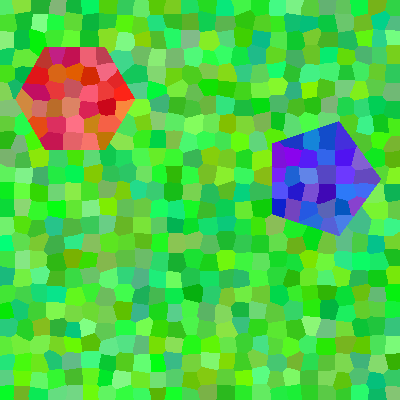
\includegraphics[width = 0.41\textwidth]{linear_coloured/train/117.png}} &
            \fcolorbox{black}{white}{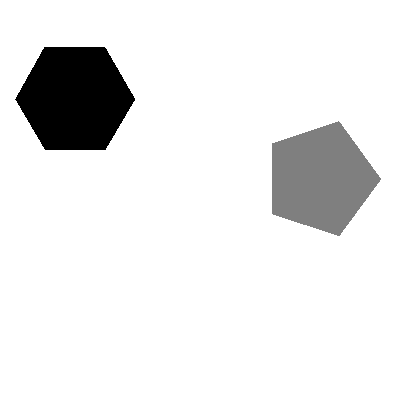
\includegraphics[width = 0.41\textwidth]{linear_coloured/result/117_N.png}}
        \end{tabular}
    \end{minipage}%
    \begin{minipage}{.5\linewidth}
        \begin{tabular}{cc}
            \fcolorbox{black}{white}{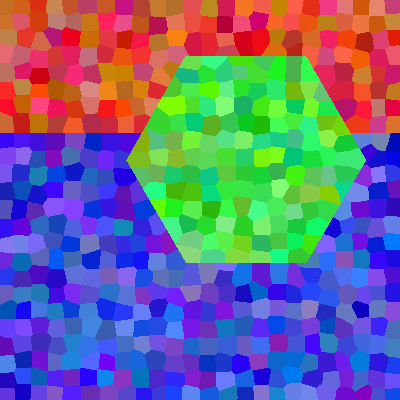
\includegraphics[width = 0.41\textwidth]{linear_coloured/train/123.png}} &
            \fcolorbox{black}{white}{
\includegraphics[width = 0.41\textwidth]{linear_coloured/result/123_N.png}} \\
            \fcolorbox{black}{white}{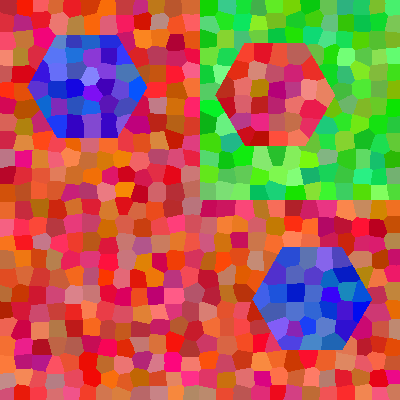
\includegraphics[width = 0.41\textwidth]{linear_coloured/train/129.png}} &
            \fcolorbox{black}{white}{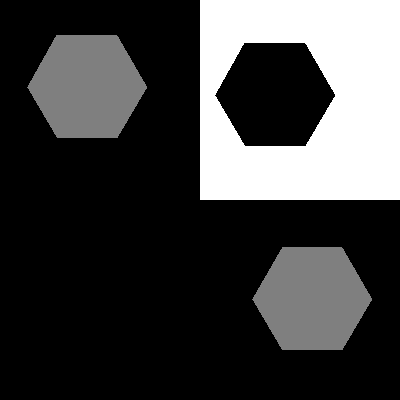
\includegraphics[width = 0.41\textwidth]{linear_coloured/result/129_N.png}} \\
            \fcolorbox{black}{white}{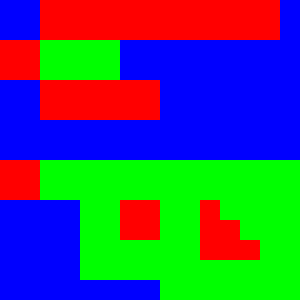
\includegraphics[width = 0.41\textwidth]{linear_coloured/train/96.png}} &
            \fcolorbox{black}{white}{
\includegraphics[width = 0.41\textwidth]{linear_coloured/result/96_N.png}}
        \end{tabular}
    \end{minipage} 
    \caption{Sample train images and their correct labellings generated for the second experiment.}
    \label{fig:training_set_coloured}
\end{figure}